\item \defpoints{20} [Math review(Information Theory)] Example of joint entropy. Let $p(x, y)$ be given by

\begin{table*}[!htbp]
    \centering
    \begin{tabular}{c|cc}
        \diagbox{$X$}{$Y$} & $0$ & $1$ \\
        \hline $0$ & $\frac{1}{3}$ & $\frac{1}{3}$  \\
        $1$ & 0 & $\frac{1}{3}$  \\
        \hline
    \end{tabular}
\end{table*}

Find:
\begin{itemize}
    \item[(a)] $H(X), H(Y)$. ~\defpoints{4}
    \item[(b)] $H(X \mid Y), H(Y \mid X)$. ~\defpoints{4}
    \item[(c)] $H(X, Y)$. ~\defpoints{3}
    \item[(d)] $H(Y)-H(Y \mid X)$. ~\defpoints{1}
    \item[(e)] $I(X ; Y)$. ~\defpoints{1}
    \item[(f)] Draw a Venn diagram for the quantities in parts (a) through (e). ~\defpoints{3}
    \item[(g)] When is the mutual information $I(X;Y)=0$?  ~\defpoints{4}
\end{itemize}

\textcolor{blue}{Solution} \\
\begin{itemize}
    \item [(a)] 
    \begin{align*}
        p(x) &= \begin{cases}
            \frac{2}{3} & x=0 \\
            \frac{1}{3} & x=1
        \end{cases} \\
        p(y) &= \begin{cases}
            \frac{1}{3} & y=0 \\
            \frac{2}{3} & y=1
        \end{cases}
    \end{align*}
    The entropy of $X$ and $Y$ are given by
    \begin{align*}
        H(X) &= -\sum_{x} p(x) \log_2 p(x) = \frac{2}{3}\log_2\frac{3}{2} + \frac{1}{3}\log_23 \\
        H(Y) &= -\sum_{y} p(y) \log_2 p(y) = \frac{1}{3}\log_23 + \frac{2}{3}\log_2\frac{3}{2}
    \end{align*}

    \item [(b)]
    $H(X \mid Y) = H(X \mid Y=0)p(Y=0) + H(X \mid Y=1)p(Y=1) = 0 + \frac{2}{3} \cdot (\frac{1}{2}\log_2 2 + \frac{1}{2}\log_2 2) = \frac{2}{3}$ \\
    \\
    $H(Y \mid X) = H(Y \mid X=0)p(X=0) + H(Y \mid X=1)p(X=1) = \frac{2}{3} \cdot (\frac{1}{2}\log_2 2 + \frac{1}{2}\log_2 2) + 0 = \frac{2}{3}$\\

    \item [(c)]
    $H(X, Y) = -\sum_{x}\sum_{y} p(x, y) \log_2 p(x, y) = -\frac{1}{3}\log_2\frac{1}{3} - \frac{1}{3}\log_2\frac{1}{3} - \frac{1}{3}\log_2\frac{1}{3} = \log_23$

    \item [(d)]
    $H(Y)-H(Y \mid X) = \frac{1}{3}\log_23 + \frac{2}{3}\log_2\frac{3}{2} - \frac{2}{3}$

    \item [(e)]
    $I(X ; Y) = H(Y) - H(Y \mid X) = \frac{1}{3}\log_23 + \frac{2}{3}\log_2\frac{3}{2} - \frac{2}{3}$

    \item [(f)]
    \begin{figure}[H]
        \centering
        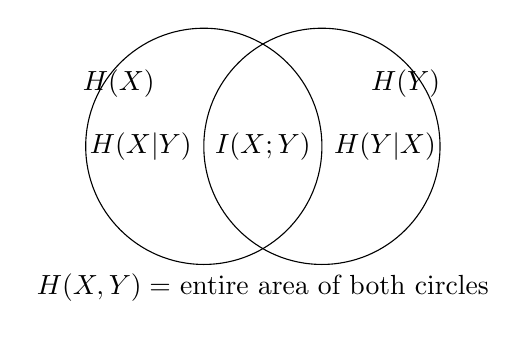
\begin{tikzpicture}
            % Draw two overlapping circles
            \def\r{1.5cm}
            \def\d{1.5cm}
            \draw (0,0) circle (\r) node[above left=0.5cm] {$H(X)$};
            \draw (\d,0) circle (\r) node[above right=0.5cm] {$H(Y)$};
            
            % Label regions
            \node at (-0.8,0) {$H(X|Y)$};
            \node at (2.3,0) {$H(Y|X)$};
            \node at (\d/2,0) {$I(X;Y)$};
            
            % Add a note about joint entropy
            \node[below=1.5cm] at (\d/2,0) {$H(X,Y) = $ entire area of both circles};
        \end{tikzpicture}
    \end{figure}

    \item [(g)]
    The mutual information $I(X;Y)=0$ when $X$ and $Y$ are independent. In this case, $p(x, y) = p(x)p(y)$.
    \begin{align*}
        I(X;Y) &= \sum_{x,y} p(x,y) \log_2 \frac{p(x,y)}{p(x)p(y)}\\
        &= \sum_{x,y} p(x,y) \log_2 \frac{p(x)p(y)}{p(x)p(y)}\\
        &= \sum_{x,y} p(x,y) \log_2 1\\
        &= \sum_{x,y} p(x,y) \cdot 0\\
        &= 0
    \end{align*}
\end{itemize}












\newpage